\def\sectiontitle{Background}

\section{\sectiontitle}

%%%%%%%%%%%%%%%%%%%%%%%%%%%%%%%%%%%%%%%%%%%%%%%%%%%%%%%%%%%%%%%%%%%%%%%%%%%%%%%%
\def\slidetitle{Problem statement}

\subsection{\slidetitle}
\begin{frame}
  \frametitle{\sectiontitle}
  \framesubtitle{\slidetitle}

  Problem
  \begin{itemize}
    \item Lower the barriers for reusing trained AI models available in AI models repositories
  \end{itemize}

  Challenges
  \begin{itemize}
    \item Scattered models in a lot of different repositories and stored in many formats
    \item It is not trivial to setup and execute AI models for non-technical researchers
    \item Re-training models from scratch take a lot of time and money
  \end{itemize}

  Motivations
  \begin{itemize}
    \item Accelerate applications of AI models to scientific problems
    \item Save computation time by reusing pre-trained models from diverse repositories
  \end{itemize}
\end{frame}

%%%%%%%%%%%%%%%%%%%%%%%%%%%%%%%%%%%%%%%%%%%%%%%%%%%%%%%%%%%%%%%%%%%%%%%%%%%%%%%%
\def\slidetitle{Related work}

\subsection{\slidetitle}
\begin{frame}
  \frametitle{\sectiontitle}
  \framesubtitle{\slidetitle}

  Already existing APIs or tools to download, inference (and train) AI models
  \begin{itemize}
    \item Transformers (Hugging Face API)*
    \item Cellpose API**
    \item BioImage.IO Core (Python libraries)
    \item SAM2 repository***
  \end{itemize}

  \bigskip
  \bigskip

  *https://aclanthology.org/2020.emnlp-demos.6/

  **https://www.biorxiv.org/content/10.1101/2020.02.02.931238v1

  ***https://arxiv.org/abs/2408.00714
\end{frame}

%%%%%%%%%%%%%%%%%%%%%%%%%%%%%%%%%%%%%%%%%%%%%%%%%%%%%%%%%%%%%%%%%%%%%%%%%%%%%%%%
\def\slidetitle{No common APIs}

\subsection{\slidetitle}
\begin{frame}[containsverbatim]
  \frametitle{\sectiontitle}
  \framesubtitle{\slidetitle}

  No common APIs/CLIs/no standard for 'download API'

  \begin{listing}[H]
    \begin{minted}[frame=lines,framesep=2mm,baselinestretch=0.8,fontsize=\footnotesize,linenos]{python}
      # BioImage.IO
      model = load_description(args.model)

      # Hugging Face
      pipe = pipeline(task="mask-generation", model=args.model,
        points_per_batch=32, device=device)

      # SAM2
      mask_generator = SAM2AutomaticMaskGenerator.from_pretrained(
        args.model, device=device)
    \end{minted}

    \begin{minted}[frame=lines,framesep=2mm,baselinestretch=0.8,fontsize=\footnotesize,linenos]{bash}
      # Cellpose
      python -m cellpose --pretrained_model cyto3
    \end{minted}
  \end{listing}

  Same problem with 'inference API', 'train API', etc

\end{frame}

%%%%%%%%%%%%%%%%%%%%%%%%%%%%%%%%%%%%%%%%%%%%%%%%%%%%%%%%%%%%%%%%%%%%%%%%%%%%%%%%
\def\slidetitle{Our approach}

\subsection{\slidetitle}
\begin{frame}
  \frametitle{\sectiontitle}
  \framesubtitle{\slidetitle}

  \begin{minipage}[h!]{0.90\textwidth}

    Our approach
    \begin{itemize}
      \item Using existing API of AI repositories
      \item Leverage WIPP
      \item Use AI model card
    \end{itemize}

    \bigskip

    Contributions
    \begin{itemize}
      \item Analyze API of AI repositories
      \item Implement them for containerized plugin that run in WIPP without learning the API
      \item Trained/Retrained AI model will comes with proper AI model card
    \end{itemize}

  \end{minipage}
\end{frame}

%%%%%%%%%%%%%%%%%%%%%%%%%%%%%%%%%%%%%%%%%%%%%%%%%%%%%%%%%%%%%%%%%%%%%%%%%%%%%%%%
\def\slidetitle{Plugin concept}

\subsection{\slidetitle}
\begin{frame}
  \frametitle{\sectiontitle}
  \framesubtitle{\slidetitle}

  \begin{minipage}[h!]{0.40\textwidth}

    Web Image Processing Pipelines
    \begin{itemize}
      \item Purpose: Measurements based on terabyte-sized images
      \item Goal: Lower the barrier to execute image analyses
    \end{itemize}

    WIPP workflow
    \begin{itemize}
      \item Sequence of plugins
    \end{itemize}

    WIPP plugin
    \begin{itemize}
      \item Piece of code taking inputs/outputs and executing code
    \end{itemize}
  \end{minipage}\hfill
  \begin{minipage}[h!]{0.55\textwidth}
    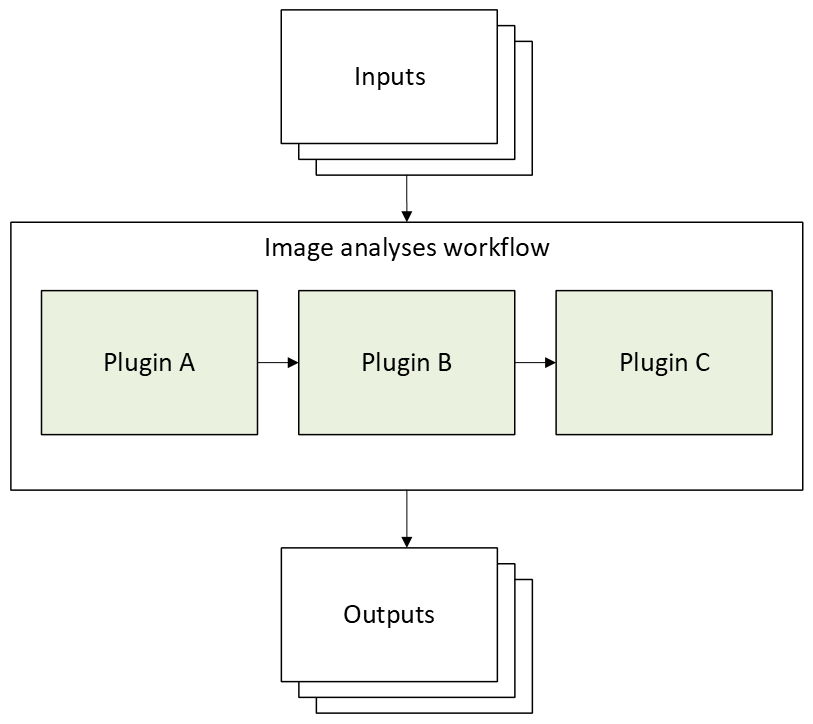
\includegraphics[scale=0.55]{./img/1_background/plugins.png}
  \end{minipage}
\end{frame}

%%%%%%%%%%%%%%%%%%%%%%%%%%%%%%%%%%%%%%%%%%%%%%%%%%%%%%%%%%%%%%%%%%%%%%%%%%%%%%%%
\def\slidetitle{AI model cards}

\subsection{\slidetitle}
\begin{frame}[containsverbatim]
  \frametitle{\sectiontitle}
  \framesubtitle{\slidetitle}

  Goal: Automatic documentation for AI models trained inside WIPP

  Work: Make AI model card proposal and development for integration

  \begin{listing}[H]
    \begin{minted}[frame=lines,framesep=2mm,baselinestretch=0.8,fontsize=\small,linenos]{java}
      public class AiModelCard {
        private String              version;
        private String              name;
        private Date                creationDate;
        private String              framework;
        private Map<String, String> trainingData;
        private Map<String, String> trainingParameters;
        [8 additional fields]
      }
    \end{minted}
    % \caption{AiModelCard.java}
  \end{listing}

  Feedback: Not relevant, AI users test directly, they don't read the documentation

\end{frame}

